\documentclass[a4paper]{article}
\usepackage{times}
\usepackage[utf8]{inputenc}
\usepackage{selinput}
\usepackage{upquote}
\usepackage[margin=2cm, rmargin=4cm, tmargin=3cm]{geometry}
\usepackage{tcolorbox}
\usepackage{xspace}
\usepackage[french]{babel}
\usepackage{url}
\usepackage{hyperref}
\usepackage{fontawesome5}
\usepackage{marginnote}
\usepackage{ulem}
\usepackage{tcolorbox}
\usepackage{graphicx}
%\usepackage[top=Bcm, bottom=Hcm, outer=Ccm, inner=Acm, heightrounded, marginparwidth=Ecm, marginparsep=Dcm]{geometry}


\newtcolorbox{Example}[1]{colback=white,left=20pt,colframe=slideblue,fonttitle=\bfseries,title=#1}
\newtcolorbox{Solutions}[1]{colback=white,left=20pt,colframe=green,fonttitle=\bfseries,title=#1}
\newtcolorbox{Conseils}[1]{colback=white,left=20pt,colframe=slideblue,fonttitle=\bfseries,title=#1}
\newtcolorbox{Warning}[1]{colback=white,left=20pt,colframe=warning,fonttitle=\bfseries,title=#1}

\setlength\parindent{0pt}

  %Exercice environment
  \newcounter{exercice}
  \newenvironment{Exercice}[1][]
  {
  \par
  \stepcounter{exercice}\textbf{Question \arabic{exercice}:} (\faClock \enskip \textit{#1})
  }
  {\bigskip}
  

% Title
\newcommand{\titre}{\begin{center}
  \section*{Algorithmes et Pensée Computationnelle}
\end{center}}
\newcommand{\cours}[1]
{\begin{center} 
  \textit{#1}\\
\end{center}
  }


\newcommand{\exemple}[1]{\newline~\textbf{Exemple :} #1}
%\newcommand{\attention}[1]{\newline\faExclamationTriangle~\textbf{Attention :} #1}

% Documentation url (escape \# in the TP document)
\newcommand{\documentation}[1]{\faBookOpen~Documentation : \href{#1}{#1}}

% Clef API
\newcommand{\apikey}[1]{\faKey~Clé API : \lstinline{#1}}
\newcommand{\apiendpoint}[1]{\faGlobe~Url de base de l'API \href{#1}{#1}}

%Listing Python style
\usepackage{color}
\definecolor{slideblue}{RGB}{33,131,189}
\definecolor{green}{RGB}{0,190,100}
\definecolor{blue}{RGB}{121,142,213}
\definecolor{grey}{RGB}{120,120,120}
\definecolor{warning}{RGB}{235,186,1}

\usepackage{listings}
\lstdefinelanguage{texte}{
    keywordstyle=\color{black},
    numbers=none,
    frame=none,
    literate=
           {é}{{\'e}}1
           {è}{{\`e}}1
           {ê}{{\^e}}1
           {à}{{\`a}}1
           {â}{{\^a}}1
           {ù}{{\`u}}1
           {ü}{{\"u}}1
           {î}{{\^i}}1
           {ï}{{\"i}}1
           {ë}{{\"e}}1
           {Ç}{{\,C}}1
           {ç}{{\,c}}1,
    columns=fullflexible,keepspaces,
	breaklines=true,
	breakatwhitespace=true,
}
\lstset{
    language=Python,
	basicstyle=\bfseries\footnotesize,
	breaklines=true,
	breakatwhitespace=true,
	commentstyle=\color{grey},
	stringstyle=\color{slideblue},
  keywordstyle=\color{slideblue},
	morekeywords={with, as, True, False, Float, join, None, main, argparse, self, sort, __eq__, __add__, __ne__, __radd__, __del__, __ge__, __gt__, split, os, endswith, is_file, scandir, @classmethod},
	deletekeywords={id},
	showspaces=false,
	showstringspaces=false,
	columns=fullflexible,keepspaces,
	literate=
           {é}{{\'e}}1
           {è}{{\`e}}1
           {ê}{{\^e}}1
           {à}{{\`a}}1
           {â}{{\^a}}1
           {ù}{{\`u}}1
           {ü}{{\"u}}1
           {î}{{\^i}}1
           {ï}{{\"i}}1
           {ë}{{\"e}}1
           {Ç}{{\,C}}1
           {ç}{{\,c}}1,
    numbers=left,
}

\newtcbox{\mybox}{nobeforeafter,colframe=white,colback=slideblue,boxrule=0.5pt,arc=1.5pt, boxsep=0pt,left=2pt,right=2pt,top=2pt,bottom=2pt,tcbox raise base}
\newcommand{\projet}{\mybox{\textcolor{white}{\small projet}}\xspace}
\newcommand{\optionnel}{\mybox{\textcolor{white}{\small Optionnel}}\xspace}
\newcommand{\advanced}{\mybox{\textcolor{white}{\small Pour aller plus loin}}\xspace}
\newcommand{\auto}{\mybox{\textcolor{white}{\small Auto-évaluation}}\xspace}


\usepackage{environ}
\newif\ifShowSolution
\NewEnviron{solution}{
  \ifShowSolution
	\begin{Solutions}{\faTerminal \enskip Solution}
		\BODY
	\end{Solutions}
  \fi}


  \usepackage{environ}
  \newif\ifShowConseil
  \NewEnviron{conseil}{
    \ifShowConseil
    \begin{Conseils}{\faLightbulb \quad Conseil}
      \BODY
    \end{Conseils}

    \fi}

    \usepackage{environ}
  \newif\ifShowWarning
  \NewEnviron{attention}{
    \ifShowWarning
    \begin{Warning}{\faExclamationTriangle \quad Attention}
      \BODY
    \end{Warning}

    \fi}
  

%\newcommand{\Conseil}[1]{\ifShowIndice\ \newline\faLightbulb[regular]~#1\fi}


\usepackage{array}
\newcolumntype{C}[1]{>{\centering\let\newline\\\arraybackslash\hspace{0pt}}m{#1}}

\begin{document}
% Change the following values to true to show the solutions or/and the hints
\ShowSolutiontrue
\ShowConseiltrue
\titre
\cours{Algorithmes de recherche}


\begin{comment}
\begin{enumerate}
    \item Recherche séquentielle
    \item Recherche binaire
    \item Arbres de recherche binaire\\
\end{enumerate}
\end{comment}

Le but de cette séance est de se familiariser avec les algorithmes de recherche. Dans la série d'exercices, nous manipulerons des listes et collections en Java et Python. Nous reviendrons sur la notion de récursivité et découvrirons les arbres de recherche. Au terme de cette séance, l'étudiant sera en mesure d'effectuer des recherches de façon efficiente sur un ensemble de données.

Le code présenté dans les énoncés se trouve sur Moodle, dans le dossier \lstinline{Ressources}.


\section{Recherche séquentielle (ou recherche linéaire)}

\subsection{Définition}

Une recherche \textbf{séquentielle} (ou \textbf{linéaire}) est une méthode permettant de trouver un élément dans un ensemble de données (liste, tableau ou dictionnaire). Elle vérifie un à un chaque élément de gauche à droite jusqu'à ce qu'une correspondance soit trouvée ou que toute la liste ait été parcouru.\\

Si l'élément recherché est trouvé, l'algorithme \textbf{renvoie l'index}, c'est-à-dire la position, de l'élément dans l'ensemble de données. \\

Sa complexité dans le pire des cas est de \textbf{O(n)} correspondant à la longueur de l'ensemble de données, et dans le meilleur des cas de \textbf{O(1)}, lorsque l'élément se trouve en première position. Dans la pratique, l'algorithme de recherche séquentielle est n'est pas couramment utilisé eu égard de sa complexité élevée et des alternatives de recherche plus efficaces comme la recherche binaire.\\



\subsection{Exercices}

\begin{Exercice}[5 minutes] Recherche séquentielle - 1 (Python)\\

À partir des éléments ci-dessous, écrivez une fonction qui cherche \lstinline{x} dans la liste \lstinline{L}.

La fonction doit retourner l'index de l'élément correspondant de la liste si \lstinline{x} est dans la liste et "-1" si \lstinline{x} n'est pas dans la liste (avec \lstinline{x = 100}).\\

\textbf{Python :}
  \lstinputlisting{resources/question1.py}

\begin{conseil}
    Définissez votre fonction de recherche linéaire en utilisant une boucle \lstinline{for} ou une boucle \lstinline{while}.\\\\
    Attention: la fonction doit retourner l'index de la valeur et non pas la valeur. Pour cela, pensez à utiliser \lstinline{range(len(list))} avec la boucle \lstinline{for} et une incrémentation \lstinline{"i = i+1"} avec la boucle \lstinline{while}.\\\\
    Utilisez la fonction \lstinline{print()} pour afficher l'index lorsque vous l'aurez trouvé et un autre message le cas échéant. 
\end{conseil}
    
\begin{solution}
\textbf{Python :}
    \lstinputlisting{solutions/question1.py}
    
\end{solution}

\end{Exercice}

\begin{Exercice}[10 minutes] Recherche séquentielle - 2 (Python)\\

Soit une liste d’entiers non triée \lstinline{L} ainsi qu’un entier \lstinline{e}. Écrivez un programme qui retourne l'élément de la liste \lstinline{L} dont la valeur est la plus proche de \lstinline{e} en utilisant une recherche séquentielle.\\\\
Exemple :\\
L = [16, 2, 25, 8, 12, 31, 2, 56, 58, 63]\\
e = 50\\
Résultat attendu : 56\\

% TODO: add this point in the solution
Au cas où deux éléments se trouveraient à équidistance de \lstinline{e}, renvoyez l'élément le plus petit.\\

\textbf{Python :}
    \lstinputlisting{resources/question2.py}
    \begin{conseil}
        Complétez la fonction \lstinline{plus_proche_sequentielle} et exécutez le code.\\\\
        Veillez à utiliser les valeurs absolues pour comparer les différences, la plus petite pouvant être positive ou négative. En Python, la fonction \lstinline{abs()} retourne la valeur absolue. Exemple : \lstinline{abs(3-10) retourne 7}.\\\\
        Étant donné que la liste est \textbf{non triée}, l'algorithme doit obligatoirement la parcourir intégralement.\\\\
        L'algorithme doit calculer la différence entre \lstinline{e} et chaque élément de la liste \lstinline{L} en gardant toujours la plus petite différence trouvée. À la fin, il retourne l'élément de la liste correspondant à la plus petite différence.  
    \end{conseil}
    
    \begin{solution}
    \textbf{Python :}
        \lstinputlisting{solutions/question2.py}
        
    \end{solution}
    
\end{Exercice}

\begin{Exercice}[5 minutes] Recherche séquentielle - 3 (Python)\\

    Considérez une \textbf{liste d’entiers triés} \lstinline{L} ainsi qu’un entier \lstinline{e}. Écrivez un programme qui retourne l'index de l'élément \lstinline{e} de la liste \lstinline{L} en utilisant une recherche séquentielle. Si \lstinline{e} n’est pas dans \lstinline{L}, retournez -1.\\\\
    
    \begin{Example}{\faTerminal Exemple}
    L = [1231321,3213125,3284016,4729273,5492710]\\
    e = 3284016\\
    Résultat attendu: 2\\
    \end{Example}
  
\lstinputlisting{resources/question3.py}

    \begin{conseil}
        Une liste triée permet une recherche plus efficace à l'aide d'un algorithme plus simple.\\
        Retournez l'index de la valeur dans la liste. Pensez à utiliser la fonction \lstinline{index()} qui retourne l'index d'un élément au sein d'une liste en Python.\\Exemple et syntaxe: \lstinline{lst.index(i)} va indiqué la position de l'élément \lstinline{i} dans la liste \lstinline{lst}.
    \end{conseil}


    \begin{solution}
        \textbf{Python :}
        \lstinputlisting{solutions/question3.py}
    \end{solution}
\end{Exercice}

\newpage
\section{Recherche binaire}

\subsection{Définition}

Le but de la recherche binaire est de trouver l'élément recherché de façon optimale. Pour cela, il est nécessaire d'utiliser \textbf{une liste d'éléments triés}.\\

La complexité de l'algorithme de recherche binaire est \lstinline{O(log n)}. Cependant, il ne faut pas oublier le coût lié à l'obtention d'une liste triée à partir d'une liste non triée.\\

L'algorithme de recherche binaire divise l'intervalle de recherche par deux à chaque itération jusqu'à ce qu'il trouve l'élément \lstinline{x} ou que l'intervalle soit vide.\\

Ainsi, si \lstinline{x} est plus petit que l'élément du milieu, l'algorithme va choisir la moitié de gauche comme intervalle de recherche et ainsi de suite. Si \lstinline{x} est plus grand que l'élément du milieu la recherche va se faire dans la moitié droite de l'intervalle.\\

La recherche binaire se base sur les comparaisons d'ordre, alors que la recherche séquentielle se base les comparaisons d'égalité pour trouver l'élément recherché.\\

\subsection{La récursivité}

Une fonction récursive est une fonction qui s'appelle elle-même pendant son exécution. Vous trouverez ci-dessous un exemple de fonction récursive utilisée pour effectuer un calcul factoriel.\\\\
(Rappel : 4! = 4 x 3 x 2 x 1 = 24)\\

\lstinputlisting{resources/factorielle.py}

Les fonctions récursives sont courantes en informatique car elles permettent aux programmeurs d'écrire des programmes efficaces en utilisant une quantité minimale de code. Leur principal inconvénient est le fait qu'elles peuvent provoquer des exécutions infinies et d'autres résultats inattendus si elles ne sont pas écrites correctement. Si la fonction n'inclut pas les cas permettant d'arrêter la récursivité, celle-ci se répétera à l'infini, provoquant le plantage du programme ou, pire encore, l'arrêt de tout le système informatique.\\
   
\subsection{Exercices}

\begin{Exercice}[20 minutes] Récursivité et itération (Python)\\

À partir de la liste d'éléments \textbf{triés} ci-dessous, écrivez premièrement \textbf{une fonction récursive} puis \textbf{une fonction itérative} qui cherche \lstinline{x} dans la liste. La fonction doit retourner \textbf{l'index} de l'élément correspondant de la liste si \lstinline{x} est dans la liste et \lstinline{-1} dans le cas contraire.\\
Ici, \lstinline{x = 5}.\\

\textbf{Question 4.1 - Version récursive}
\lstinputlisting{resources/question4_1.py}

\textbf{Question 4.2 - Version itérative}
\lstinputlisting{resources/question4_2.py}


    \begin{conseil}
        Complétez la fonction récursive \lstinline{recherche_binaire_recursive} et la fonction itérative \lstinline{recherche_binaire_iterative}.\\\\
        Détails sur les arguments de la fonction:\\
        \lstinline{L} : La liste dans laquelle nous effectuons la recherche.\\
        \lstinline{s} : L' élément de départ de la partie de la liste à fouiller (0 au départ).\\
        \lstinline{r} : Le dernier élément de la partie de la liste à fouiller (len(liste) au départ).\\
        \lstinline{x} : La valeur recherchée.\\

        Ainsi, à chaque itération, vos fonctions vont modifier les valeurs de base données en argument pour resserrer l'intervalle jusqu'à trouver la valeur recherchée.\\        
        Pour définir le milieu d'un intervalle qui contient un nombre pair ou impair d'éléments, divisez l'ensemble en 2 et utilisez la fonction \lstinline{int()} pour convertir le résultat en entier. \\
        Exemple:\\
            liste1 = [1,2,3,4,5]\\
            s = 0\\
            r = len(liste1)\\
            Calcul du milieu de l'intervalle:\\
            (s+r)/2) = (0+5)/2 = 2.5 \#Pas de correspondance\\
            int((s+r)/2) = int((0+5)/2) = int(2.5) = 2 \\
            Arrondi vers le bas
        \\
        
        Pour la version itérative, il est conseillé d'utiliser une boucle \lstinline{while}.

    \end{conseil}

    \begin{solution}
        \textbf{4.1 - Version récursive}
        \lstinputlisting{solutions/question4-1.py}
    \end{solution}
    \begin{solution}
        \textbf{4.2 - Version itérative}
        \lstinputlisting{solutions/question4-2.py}
    \end{solution}

\end{Exercice}


\begin{Exercice}[15 minutes] Recherche binaire - plus proche élément (Python)\\

Soit une liste d’entiers \textbf{triés} \lstinline{L} ainsi qu’un entier \lstinline{e}. Écrivez un programme retournant la valeur dans \lstinline{L} la plus proche de \lstinline{e} en utilisant une recherche binaire (binary search).\\

Résultat attendu : 56\\

\lstinputlisting{resources/question5.py}

\begin{conseil}
    Pensez à définir des variables \lstinline{min} et \lstinline{max} délimitant l'intervalle de recherche et une variable booléenne \lstinline{found} initialisée \lstinline{false} et qui devient \lstinline{true} lorsque l'algorithme a trouvé la valeur la plus proche de \lstinline{e}. 
    
\end{conseil}

    \begin{solution}
        \textbf{Python :}
        \lstinputlisting{solutions/question5.py}
    \end{solution}

\end{Exercice}

\begin{Exercice}[10 minutes] Recherche binaire (Python)\\

Considérez une liste d’entiers triés \lstinline{L} ainsi qu’un entier \lstinline{e}. Écrivez un programme qui retourne l'index de l'élément \lstinline{e} de la liste L en utilisant une recherche binaire. Si \lstinline{e} n’est pas dans \lstinline{L}, retournez \lstinline{-1}.\\\\

\begin{Example}{\faTerminal \quad Exemple}
    L = [1231321,3213125,3284016,4729273,5492710] \\

    e = 3284016\\

Résultat attendu: 2
\end{Example}

\lstinputlisting{resources/question6.py}

\begin{conseil}
    Inspirez-vous des exercices et des conseils précédents. 
\end{conseil}

    \begin{solution}
        \textbf{Python :}
        \lstinputlisting{solutions/question6.py}
    \end{solution}

\end{Exercice}


\begin{Exercice}[20 minutes] Recherche matricielle (Python) \optionnel\\
    
    \textbf{Matrice en Python}

    Considérez une matrice ordonnée \lstinline{m} et un élément \lstinline{l}.\\
    
    Pour rappel, une matrice ordonnée répond aux critères suivants :\\
     \lstinline{[i][j]<=m[i+1][j]} (une ligne va du plus petit au plus grand)\\
     \lstinline{[i][j]<=m[i][j+1]} (une colonne va du plus petit au plus grand)\\
 
    
    Écrivez un algorithme qui retourne la position de l’élément \lstinline{l} dans \lstinline{m}. Si \lstinline{l} n’est pas présent dans \lstinline{m} alors il faut retourner \lstinline{(-1, -1)}\\
    
    \begin{Example}{\faTerminal \quad Exemples}
        \textbf{Exemple 1}: si m=[[1,2,3,4],[4,5,7,8],[5,6,8,10],[6,7,9,11]] et que l=7. Nous souhaitons avoir la réponse (1,2) OU (3,1) (l’une des deux, pas besoin de retourner les deux résultats).\\

        \textbf{Exemple 2}: si m=[[1,2],[3,4]] et que l=7. Nous souhaitons avoir la réponse (-1,-1) car 7 n’est pas dans la matrice m.
    \end{Example}

    \lstinputlisting{resources/question7.py}

    \begin{conseil}
    Pour cet exercice, il est nécessaire d'utiliser des boucles \lstinline{for} imbriquées, c'est-à-dire: une boucle \lstinline{for} dans une autre boucle \lstinline{for}. Cela permet de parcourir tous les éléments d'une liste (ou d'un tableau) à deux dimensions (dans notre cas une matrice). 
    \end{conseil}

    \begin{solution}
        \textbf{Python :}
        \lstinputlisting{solutions/question7.py}
    \end{solution}

\end{Exercice}

\newpage
\section{Arbre de recherche binaire}
\subsection{Définition}

Un arbre de recherche binaire est une structure de données au même titre que les listes, tuples, dictionnaires, etc. Leur particularité est qu'au lieu d'ordonner les éléments les uns à la suite des autres, les arbres de recherche binaire enregistrent les valeurs de manière relationnelle.\\

En effet, l'arbre est divisé en branches qui peuvent elles-même contenir deux branches (enfants) et ainsi de suite. Lorsqu'une branche n'a pas de branches subséquentes (enfants), on parle de feuille.\\

Les branches peuvent donc contenir de 0 à 2 autres branches. On parle alors de branche de gauche et de celle de droite. La branche de gauche est forcément plus petite que la branche parente et celle de droite est forcément plus grande.\\

De cette façon, on garantit que l'arbre est toujours ordonné même en rajoutant ou en retirant des éléments\\

\begin{figure}[h]
    \centering
    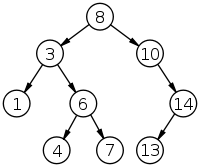
\includegraphics[width=0.32\textwidth]{img/binary-search-tree.png}
    \caption{Exemple d'arbre binaire}
\end{figure}

\subsection{Exercices}

\begin{Exercice}[15 minutes] language : \textbf{Python}\\
    
    Dans l'exercice suivant, nous vous donnons un arbre binaire avec les mêmes valeurs que le schéma précédent et dont la racine est la variable \lstinline{root}.\\

    Écrivez une fonction qui retourne \lstinline{True} si la valeur valeur est dans l'arbre et \lstinline{False} dans le cas contraire. Vous pouvez utiliser la variable \lstinline{value} pour afficher la valeur d'un nœud (\lstinline{node}) et les variables \lstinline{left} et \lstinline{right} sur les \lstinline{nodes} pour accéder aux branches enfants, utilisez \lstinline{node.value}, \lstinline{node.left} et \lstinline{node.right}.\\\\
    Complétez la fonction \lstinline{recherche_arbre}.\\
    \begin{lstlisting}[language=Python]
    import sys
    import traceback

    def recherche_arbre(node, value):
        # Complétez ici
        
        
    #Attention à inclure les lignes de codes additionnelles présentes dans le fichier "question8.py" sur Moodle
    \end{lstlisting}

    \begin{conseil}
    Indice: Utilisez une fonction récursive.\\
    
    Pour cette question, vous devez télécharger le fichier \textbf{"question8.py"} sur moodle et copier tout son contenu dans votre fichier python. Celui-ci contient les classes permettant de définir les arbres selon le concept vu en cours. \\
    
    Il contient également un code de "vérification". Celui-ci va automatiquement tester votre fonction avec différent paramètres et vérifier si les résultats obtenus correspondent au résultats attendus.
    \end{conseil}

    \begin{solution}
        \textbf{Python :}
        \lstinputlisting{solutions/question8.py}
    \end{solution}

\end{Exercice}

\end{document}
